\chapter{Introducción} \label{ich:introduccion}

En la parte informática del presente trabajo buscamos resolver una \textbf{tarea de reconocimiento facial invariante a la edad}, por sus siglas en inglés, \textit{AIFR}. El \textbf{reconocimiento facial} es un conjunto de \textbf{técnicas biométricas} que tratan de reconocer, buscar o comprobar  la identidad de un individuo a partir de información sobre su cara \cite{informatica:definicion_face_recognition}. Normalmente esta información viene dada en forma de imágenes de la cara (fotografías, vídeo o imagen en tiempo real), pero existen técnicas para trabajar con información tomada de otro tipo de sensores (detectores de profundidad o  sensores de calor, por ejemplo). Estas técnicas tienen muchas áreas de aplicación, por mencionar algunas: videovigilancia, identificación de supuestos criminales y control de acceso a instalaciones \cite{informatica:deep_fr_survey}. Además, obtener sistemas que realicen esta tarea resulta muy interesante por su fácil despliegue en soluciones reales. Por ejemplo, colocando puestos de control que con una cámara manejen el acceso a un aeropuerto.

Además de las dificultades usuales en el campo de la visión por computador (cambios en la iluminación, cambios en la posición relativa dentro de la imagen y cambios en las características de la cámara) estas técnicas trabajan con \textbf{problemas específicos} introducidos por el reconocimiento facial (cambios en la orientación de la cara, cambios en la expresión facial y distractores faciales como pueden ser cambios en el corte de pelo, uso de gafas o gorros o uso de maquillaje). Sumado a esto, el \textit{AIFR} introduce como reto principal reconocer a una persona independientemente de las modificaciones que haya experimentado su rostro debido al paso del tiempo y el envejecimiento. En la \imgref{img:ejemplo_dificultad_aifr} quedan de manifiesto estas dificultades, en las que posteriormente profundizaremos.

\begin{figure}[h]
	\centering
	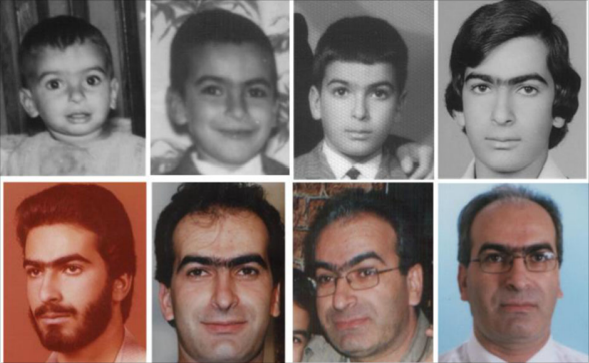
\includegraphics[width=0.8\textwidth]{informatica/ejemplo_dificultad_aifr}
	\caption{Ejemplo de datos con los que trabajamos en una tarea de \textit{AIFR}. Deja de manifiesto las dificultades específicas a las que nos enfrentamos. Principalmente cambios en las características de la cámara y los cambios faciales introducidos por el envejecimiento. Imagen extraída de \cite{informatica:aifr_survey}.}
	\label{img:ejemplo_dificultad_aifr}
\end{figure}

Estas técnicas pueden emplearse en la búsqueda de personas desaparecidas, identificación de supuestos criminales en casos en los que haya pasado mucho tiempo desde los sucesos investigados o que hayan cometido delitos en distintos momentos de su vida y verificación de documentos de identidad como pasaportes \cite{informatica:aifr_survey}.

Para resolver las dificultades que un problema de visión por computador plantea, las técnicas de aprendizaje profundo han surgido como el enfoque más prometedor superando otros enfoques clásicos. Además de haber destacado históricamente en el groso de los problemas de visión por computador, han probado su valía específicamente en tareas de reconocimiento facial \cite{informatica:deep_fr_survey} y tareas de \textit{AIFR} \cite{informatica:aifr_survey}. Comentamos brevemente algunas de las características fundamentales de las redes profundas, que las hace adecuadas para trabajar en tareas de visión por computador:

\begin{itemize}
	\item Representación jerárquica de las características: estos modelos son capaces de reconocer características de alto nivel sobre las imágenes, y en específico, sobre los rostros. Por tanto parece que serán capaces de realizar mejores razonamientos sobre estos tipos de datos.
	\item La extracción de características (en nuestro problema a tratar, características faciales) se aprende a partir de los datos. No dependemos de un experto que diseñe los métodos para extraer dichas características.
	\item Gracias al uso de grandes conjuntos de datos podemos aprender modelos mucho más expresivos que con otros métodos, como por ejemplo, comparación de características faciales diseñadas a mano.
\end{itemize}

Aunque todavía no hemos introducido los fundamentos técnicos sobre los que se basa nuestro trabajo, cabe destacar que una \textbf{parte fundamental de este consiste en explorar cierta modificación técnica en una de las piezas de nuestra solución}. Dicho estudio se realiza en la \sectionref{isec:mejoras_tecnicas_objeto_de_estudio}. Del mismo modo, aunque detallaremos ciertos conceptos técnicos en la \sectionref{isec:github_buenas_practicas}, es relevante señalar ahora que todo el desarrollo del código y la creación de esta memoria se ha llevado a cabo en un repositorio público alojado en \textbf{\textit{GitHub}} \cite{informatica:repogithub}. En este repositorio, se encuentran disponibles los registros de todos los cambios o \textit{commits}, introducción de cambios a la rama principal usando \textit{pull requests}, documentación de problemas y nuevas funcionalidades a través de \textit{issues}, ramas de desarrollo usando \textit{feature branches} y la integración continua a través de \textit{GitHub Actions}.

\section{Descripción del problema} \label{ich:descrp_problema}

Como ya se ha comentado, este trabajo estudia un problema de \textit{AIFR}. Recordemos que el reconocimiento facial es una rama de la biometría que se centra en identificar individuos a partir de su rostro y que ha demostrado su utilidad en diversas aplicaciones, como la videovigilancia, la identificación de posibles criminales y el control de acceso a instalaciones. El \textit{AIFR} introduce desafíos adicionales al lidiar con los cambios que el envejecimiento provoca en las características faciales. En esta sección nos centraremos en presentar tanto las dificultades generales que presenta un problema de reconocimiento facial como las dificultades específicas del \textit{AIFR}. Empecemos viendo las tareas concretas en las que se puede categorizar un problema de reconocimiento facial:

\begin{itemize}
	\item \textbf{\textit{Retrieval}} o búsqueda: dada una imagen de una persona objetivo y una base de datos de imágenes, devolver un número específico de imágenes tomadas de la base de datos de la persona objetivo. Esta es la tarea que intentamos resolver en el presente trabajo \footnotemark.

	      \begin{itemize}
		      \item Por ejemplo, tras la desaparición de una persona, tomar imágenes de distintas bases de datos policiales y estudiar las 100 imágenes con mayor probabilidad de corresponderse con la identidad de la persona desaparecida.
		      \item A la acción de aportar una imagen, una base de datos y devolver las $N$ imágenes más probables de coincidir en la identidad de la persona de la primera imagen se le conoce como consulta o \textit{query}. A la imagen pasada como parámetro se le conoce como \textit{key} o llave.
	      \end{itemize}

	\item \textbf{Verificación}: dadas dos imágenes, el modelo debe decidir si se trata de la misma persona o no. Por ejemplo, en un aeropuerto, comprobar la imagen del pasaporte y la imagen obtenida de las cámaras de los puestos de control \cite{informatica:docface}.
\end{itemize}

\footnotetext{Por lo tanto, realmente nuestra tarea consiste en realizar búsqueda de imágenes faciales invariante a cambios en la edad. En adelante, salvo que induzca a confusión, nos referiremos a esta tarea implemente como \textit{AIFR}.}


La \imgref{img:ejemplo_verificacion} explica visualmente la tarea de verificación, mientras que la \imgref{img:ejemplo_retrieval} explica la tarea de \textit{retrieval}:

\begin{figure}[H]
	\centering
	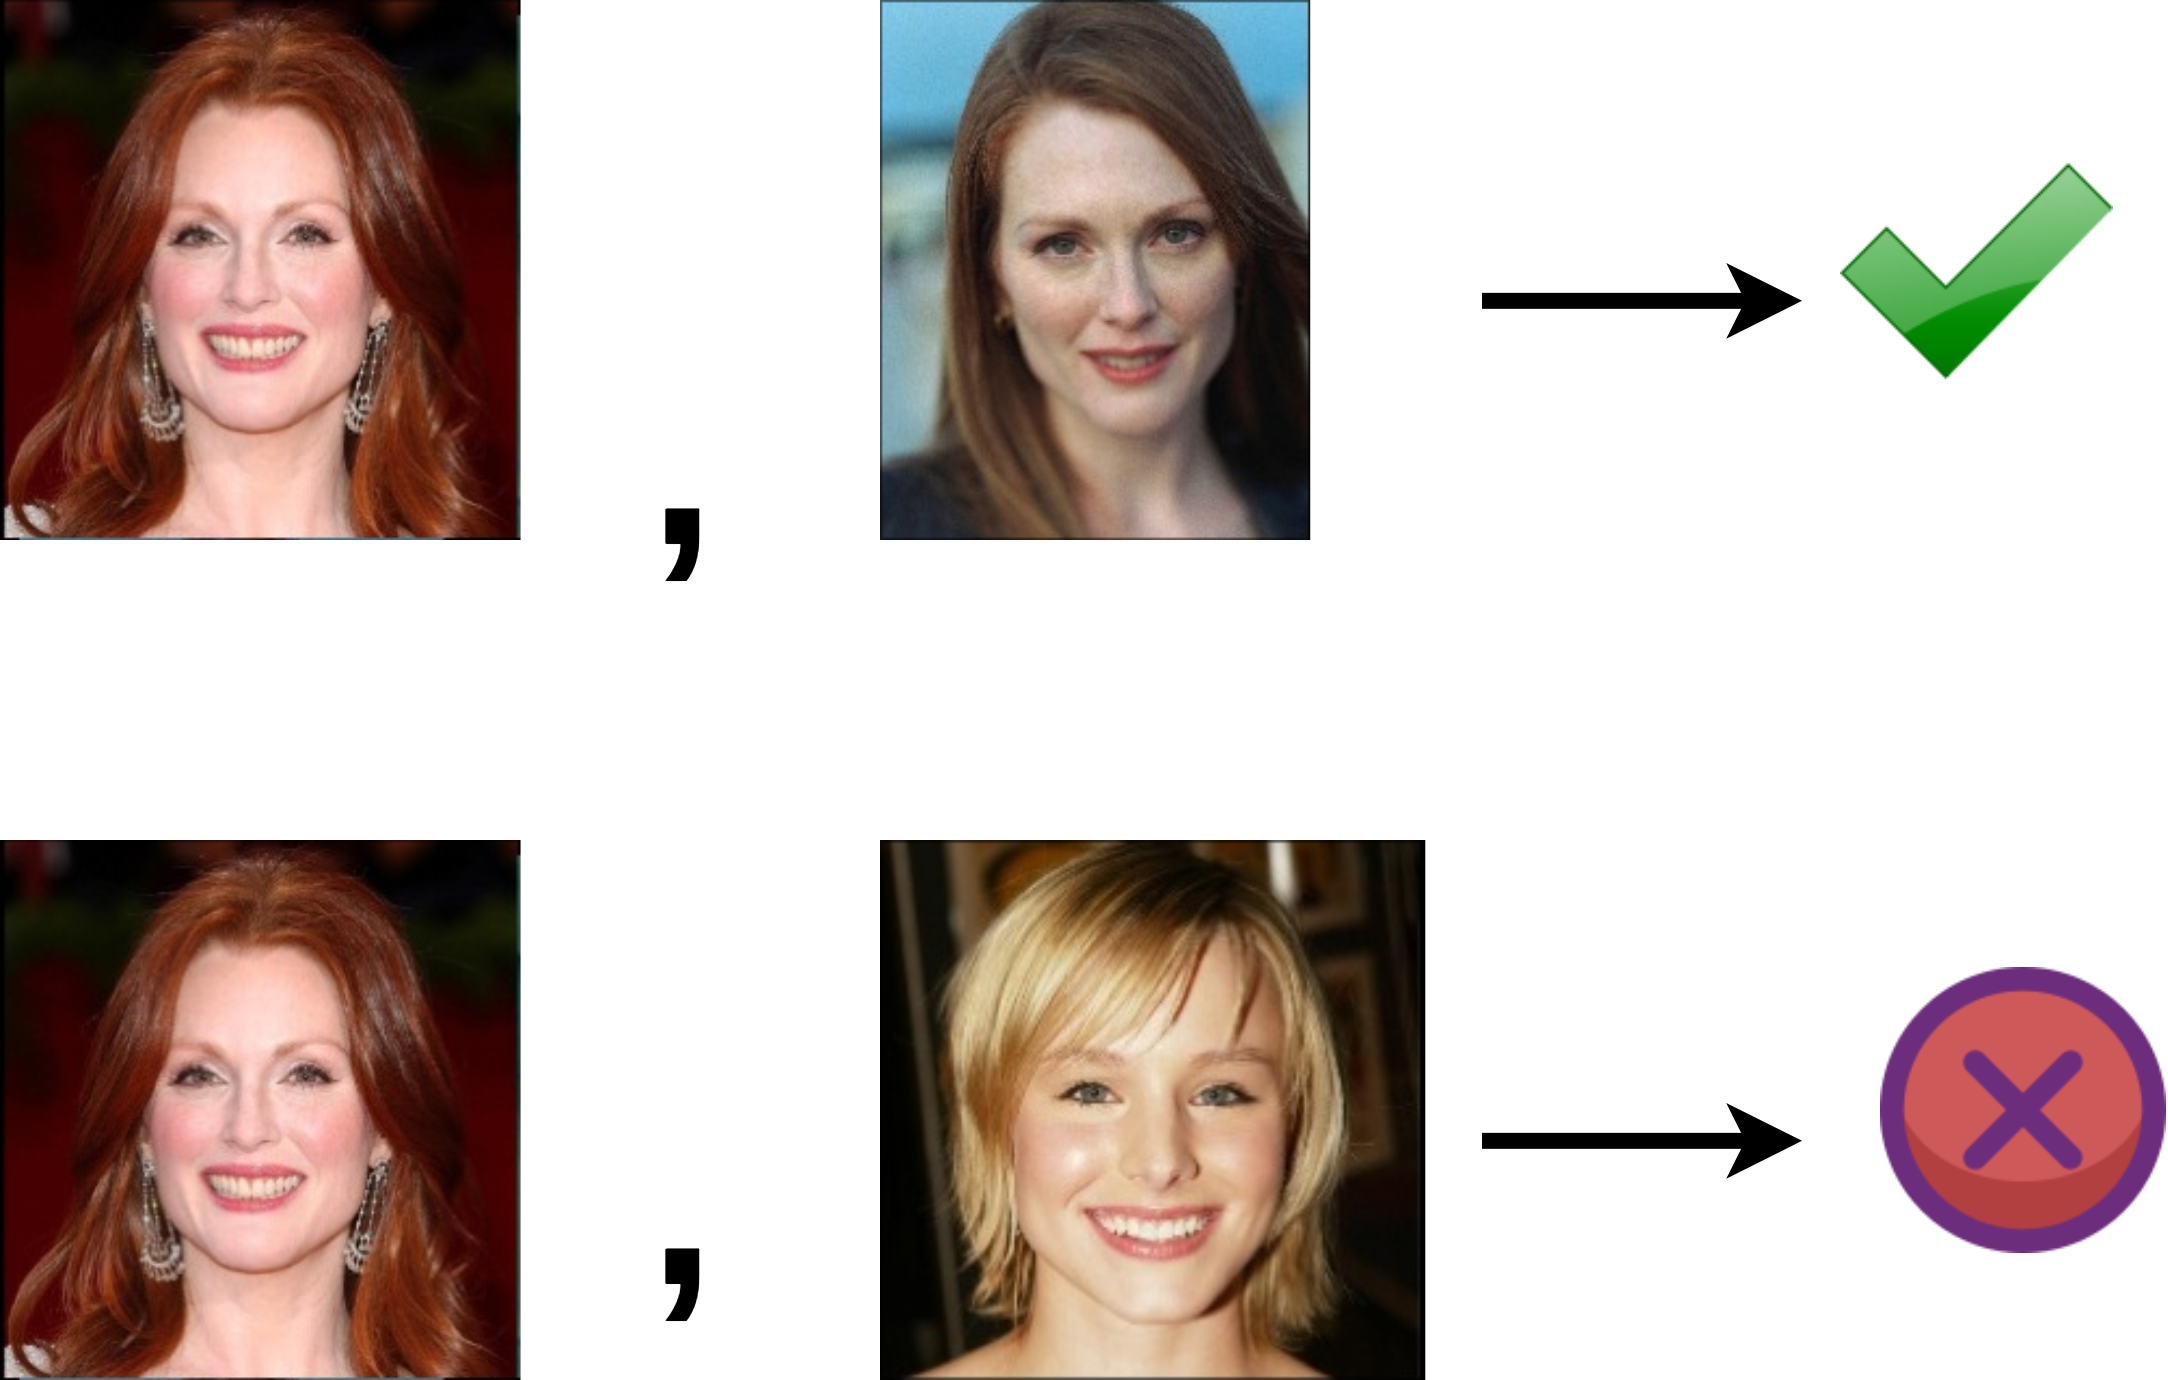
\includegraphics[width=0.5\textwidth]{informatica/ejemplos_tareas/verification}
	\caption{Ejemplo gráfico de la tarea de verificación. Dado un par de imágenes, decidimos si se corresponden a la misma identidad o si son dos personas distintas. Imágenes extraídas de \cite{informatica:cacd_dataset}.}
	\label{img:ejemplo_verificacion}
\end{figure}

\begin{figure}[H]
	\centering
	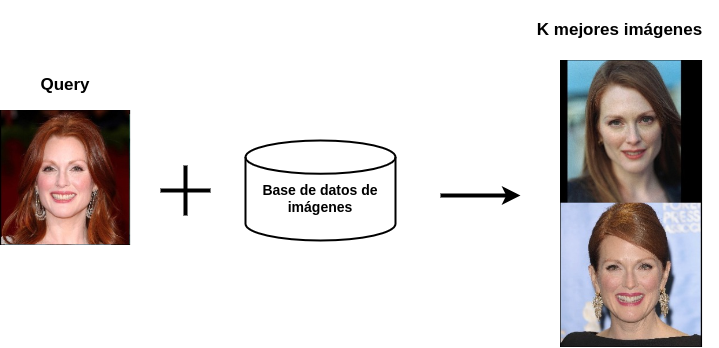
\includegraphics[width=0.7\textwidth]{informatica/ejemplos_tareas/retrieval}
	\caption{Ejemplo gráfico de la tarea de búsqueda. Dada una imagen objetivo y una base de datos de imágenes candidatas, devolvemos las mejores $K = 2$ imágenes. Imágenes extraídas de \cite{informatica:cacd_dataset}.}
	\label{img:ejemplo_retrieval}
\end{figure}

Por otro lado, nos enfrentamos a las siguientes \textbf{dificultades específicas del \textit{AIFR}} \cite{informatica:challenges_retrieval}:

\begin{itemize}
	\item \textbf{Invarianzas}: en nuestro problema esto es especialmente relevante. Al trabajar con imágenes tomadas en instantes de tiempo muy variados, las características de la imagen pueden variar considerablemente. Pensemos, por ejemplo, en fotografías antiguas que fueron tomadas en blanco y negro, en contraste con fotografías más actuales en color. O cambios considerables en características de la cámara con la que se toman las fotografías.

	\item Problemas asociados al \textbf{envejecimiento}: cómo varía la cara con el paso de los años es un proceso muy complejo. Algunos de los factores que afectan a este envejecimiento \cite{informatica:tecnica_sintesis_aifr} son los factores intrínsecos (genética, etnia) y factores extrínsecos (ambiente o hábitos de vida). Además, algunas características de la cara cambian drásticamente con el paso de los años, como por ejemplo, la textura (aparición de arrugas, lunares y vello) o cambios en la forma de la cara (cambio en el peso corporal).

	\item Tenemos que trabajar con \textbf{identidades que nunca hemos visto} en nuestros datos de entrenamiento. En otras tareas, como por ejemplo la de clasificación de objetos cotidianos, ocurre algo parecido. Por ejemplo, tenemos imágenes de coches que nuestro modelo no ha visto durante el entrenamiento. Sin embargo la diferencia radica en que en nuestro problema el modelo debe saber identificar identidades, mientras que en el modelo de clasificación este debe saber identificar categorías.

	\item Nuestro modelo debe identificar como similares imágenes de la misma persona, aunque sea en momentos muy distintos. Y debe identificar como no similares imágenes de personas distintas. Es muy fácil que ocurra que dos imágenes de la misma persona tomadas con muchos años de diferencia parezcan más distintas que dos imágenes de dos personas distintas pero de la misma edad. Por ejemplo, esto se puede ver en la \imgref{img:messi_distintos_otro_adulto} \footnote{El concepto de similitud con el que codificamos la identidad de los sujetos lo especificamos en \customref{isec:embeddings})}.

	\item Aunque desarrollemos esto más tarde en la \sectionref{isec:base_datos_usada}, los \textbf{\textit{datasets} de \textit{AIFR} son escasos y presentan problemas} \cite{informatica:tecnica_sintesis_aifr}. Algunas de estas bases de datos son muy pequeñas. Otras, son de un tamaño más grande, pero presentan mucha menos variabilidad en los rangos de edad. Y por supuesto, muchas de estas bases de datos presentan problemas de representatividad (etnia, sexo).

	\item \textbf{Eficiencia}: aunque este es un problema generalizado en todas las soluciones basadas en aprendizaje profundo, los problemas de eficiencia se vuelven más acuciantes en el \textit{AIFR}. Principalmente porque a la hora de que nuestro modelo reciba una consulta, desconocemos el tamaño de la base de datos sobre la que tenemos que operar.
\end{itemize}

Las imágenes presentadas en la \imgref{img:messi_cuatro_edades} son un buen ejemplo de los problemas específicos que acabamos de comentar. Por ejemplo, la imagen en la que aparece siendo más pequeño, \ref{img:messi_pequeno}, es de una calidad mucho menor que el resto de imágenes. No ha desarrollado todavía rasgos faciales muy característicos. La variabilidad en el estilo de pelo es total. Se puede apreciar perfectamente cómo el paso de los años va modificando los rasgos de la cara. Y todo esto sin comentar problemas comunes y bien conocidos en la visión por computador como cambios en la pose, cambios en la iluminación o aparición de distractores. Por ejemplo, en la fotografía \ref{img:messi_adulto} podemos ver que, en el fondo de la imagen, aparece otro jugador, y nuestro modelo podría distraerse por este hecho.

\begin{figure}[H]
	\centering
	\begin{subfigure}{0.5\textwidth}
		\centering
		\includegraphics[width=0.5\linewidth]{informatica/messi_niño}
		\caption{Edad temprana. Imagen extraída de \cite{informatica:webimg_messi_pequeno}}
		\label{img:messi_pequeno}
	\end{subfigure}%
	\begin{subfigure}{.5\textwidth}
		\centering
		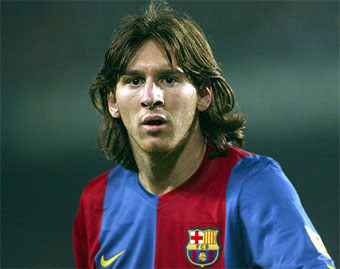
\includegraphics[width=0.8\linewidth]{informatica/messi_joven}
		\caption{Edad joven. Imagen extraída de \cite{informatica:webimg_messi_joven}}
	\end{subfigure}%

	\begin{subfigure}{.5\textwidth}
		\centering
		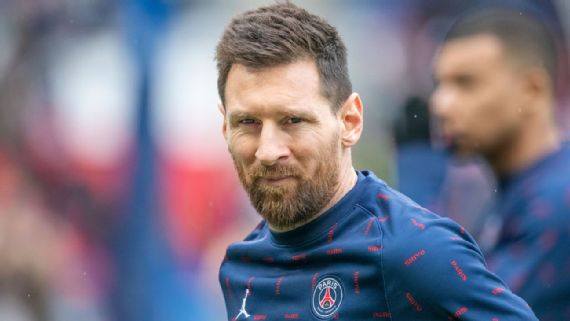
\includegraphics[width=0.6\linewidth]{informatica/messi_adulto}
		\caption{Edad adulta. Imagen extraída de \cite{informatica:webimg_messi_adulto}}
		\label{img:messi_adulto}
	\end{subfigure}%
	\begin{subfigure}{.5\textwidth}
		\centering
		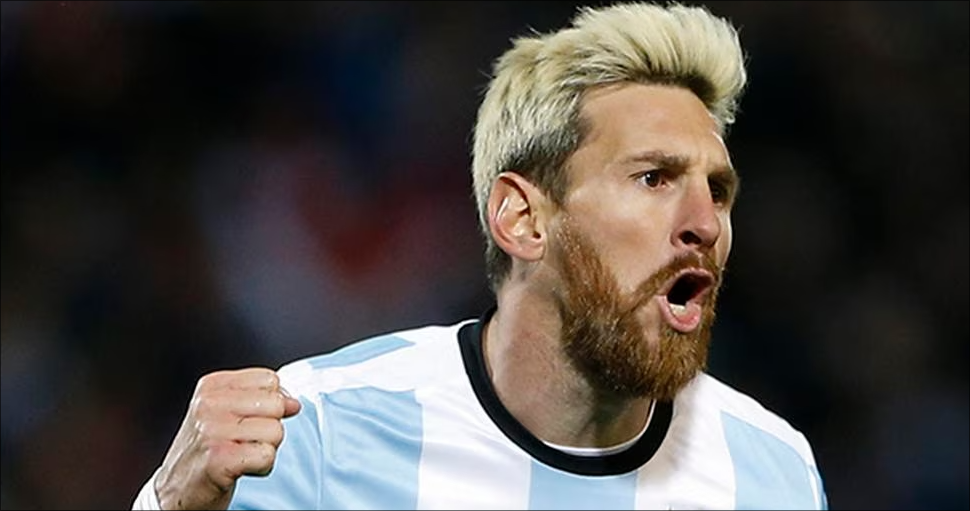
\includegraphics[width=0.8\linewidth]{informatica/messi_rubio}
		\caption{Otra imagen en la edad adulta, pocos años después. Imagen extraída de \cite{informatica:webimg_messi_rubio}}
	\end{subfigure}

	\caption{Lionel Messi en cuatro momentos distintos de su vida}
	\label{img:messi_cuatro_edades}

\end{figure}
\todo{Conseguir que las cuatro imágenes tengan el mismo tamaño y misma relación de aspecto}

\begin{figure}[hbtp]
	\centering
	\begin{subfigure}{0.5\textwidth}
		\centering
		\includegraphics[width=0.4\linewidth]{informatica/messi_niño}
		\caption{Messi en una edad temprana}
	\end{subfigure}%
	\begin{subfigure}{.5\textwidth}
		\centering
		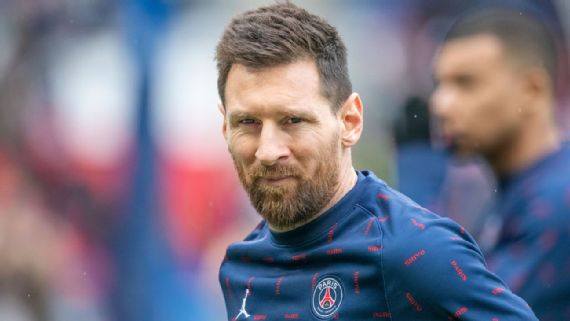
\includegraphics[width=0.8\linewidth]{informatica/messi_adulto}
		\caption{Messi en edad adulta}
	\end{subfigure}

	\begin{subfigure}{.6\textwidth}
		\centering
		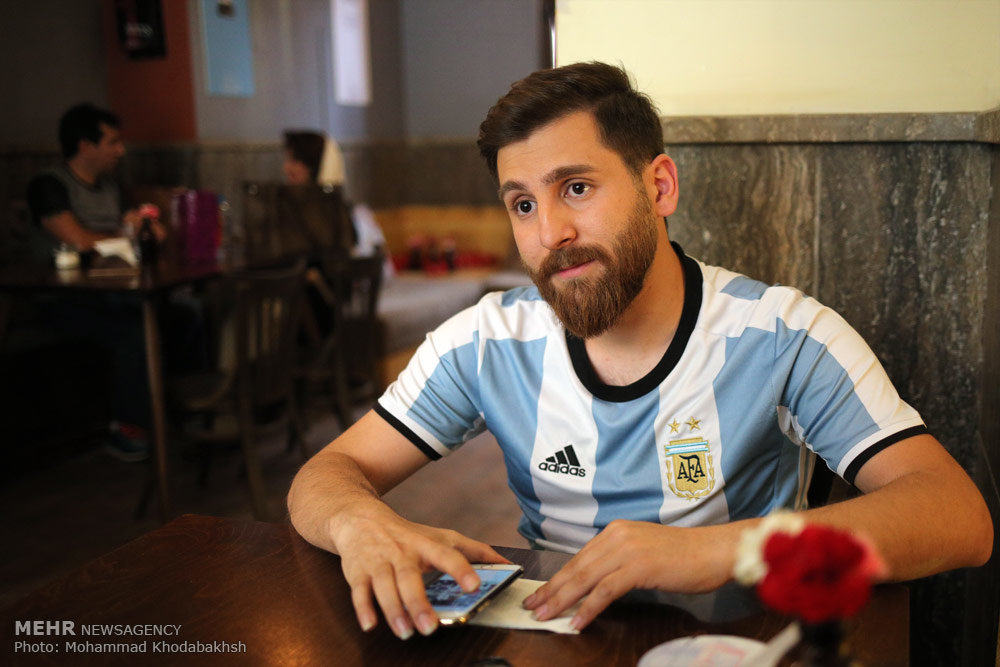
\includegraphics[width=0.6\linewidth]{informatica/doble_messi}
		\caption{Riza Perestes, ciudadano iraní. Imagen extraída de \cite{informatica:imitador_messi}}
	\end{subfigure}

	\caption{Lionel Messi en dos momentos distintos de su vida, y Riza Perestes, ciudadano iraní con gran parecido}
	\label{img:messi_distintos_otro_adulto}
\end{figure}

Ahora estudiemos el ejemplo presentado en la \imgref{img:messi_distintos_otro_adulto}. En este ejemplo vemos un problema que hemos comentado previamente: tenemos más parecido entre dos personas distintas pero de la misma edad, que entre la misma persona pero a distintas edades. En este caso el parecido es extraordinario, pero es razonable que nuestro modelo tenga dificultades en asignar mayor parecido a imágenes de la misma persona en su adultez y niñez, que a imágenes de dos personas distintas, ambas con barba y mismo corte de pelo.

Y para finalizar, introducimos los \textbf{dos enfoques principales usados para resolver problemas de \textit{AIFR}}, que estudiaremos en profundidad en  el \sectionref{ich:estado_arte}. El \textbf{primer enfoque} es aplicar modelos generativos adversarios (\textit{GAN}). Por ejemplo, el \textit{Age Invariant Model} o \textit{AIM} propuesto en \cite{informatica:tecnica_sintesis_aifr}. El \textbf{segundo enfoque} es directamente trabajar sobre una base de datos que presente la suficiente variabilidad en la edad de los individuos, y desarrollar un modelo que realice nuestra tarea. Este enfoque casi siempre pasa por computar un \textit{embedding}. Este será el enfoque que sigamos.

\section{Motivación}

El ámbito de aplicación de un modelo de \textit{AIFR} es amplio, destacando el ámbito de la \textbf{informática forense}. La informática forense se puede definir como \entrecomillado{la disciplina de las ciencias forenses que, considerando las tareas propias asociadas a la evidencia, procura descubrir e interpretar la información en los medios informáticos para establecer los hechos y formular las hipótesis relacionadas con el caso} o como \entrecomillado{la disciplina científica y especializada que, entendiendo los elementos propios de las tecnologías de los equipos de computación, ofrece un análisis de la información residente en dichos equipos} \cite{informatica:libro_informatica_forense}.

Algunos ejemplos de aplicación son:

\begin{itemize}
	\item Reconocer caras de sospechosos que llevan en busca un tiempo en imágenes de videovigilancia.
	\item Reconocer caras de personas desaparecidas un tiempo considerable, en imágenes de videovigilancia y controles de aeropuertos.
	\item Verificación automática de documentos de identidad en puestos de control \cite{informatica:tecnica_sintesis_aifr}. Por ejemplo, los puestos de control automáticos de aeropuertos. En estos puestos, una máquina verifica que la imagen que aparece en el pasaporte coincida con una imagen tomada en ese momento con una cámara.
	\item Consultar en una base de datos policial las 10 identidades que más se parecen a la imagen de una persona dada.
\end{itemize}

Por ejemplo, en 2021 se pusieron en marcha en España máquinas \textit{ABC System} para realizar automáticamente el control de pasaportes en aeropuertos \cite{informatica:articulo_abc_system}. Una de las tareas de esta máquina es la de verificar que la fotografía que aparece en el pasaporte se corresponde con la persona que está intentando pasar el control. Esto se muestra en las siguientes imágenes:

\begin{figure}[H]
	\centering
	\begin{subfigure}{0.4\textwidth}
		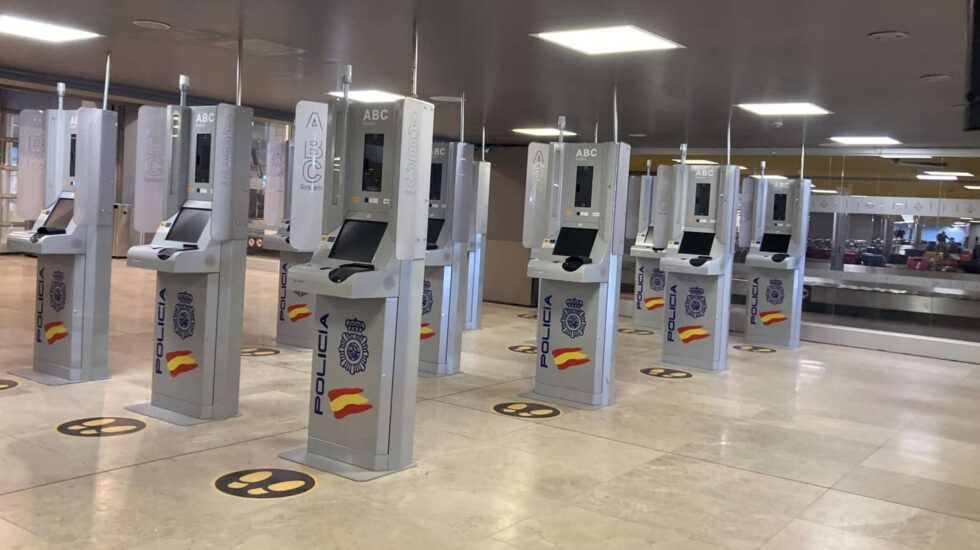
\includegraphics[width=1.0\textwidth]{informatica/ejemplo_abc_system_01}
	\end{subfigure}
	\begin{subfigure}{0.4\textwidth}
		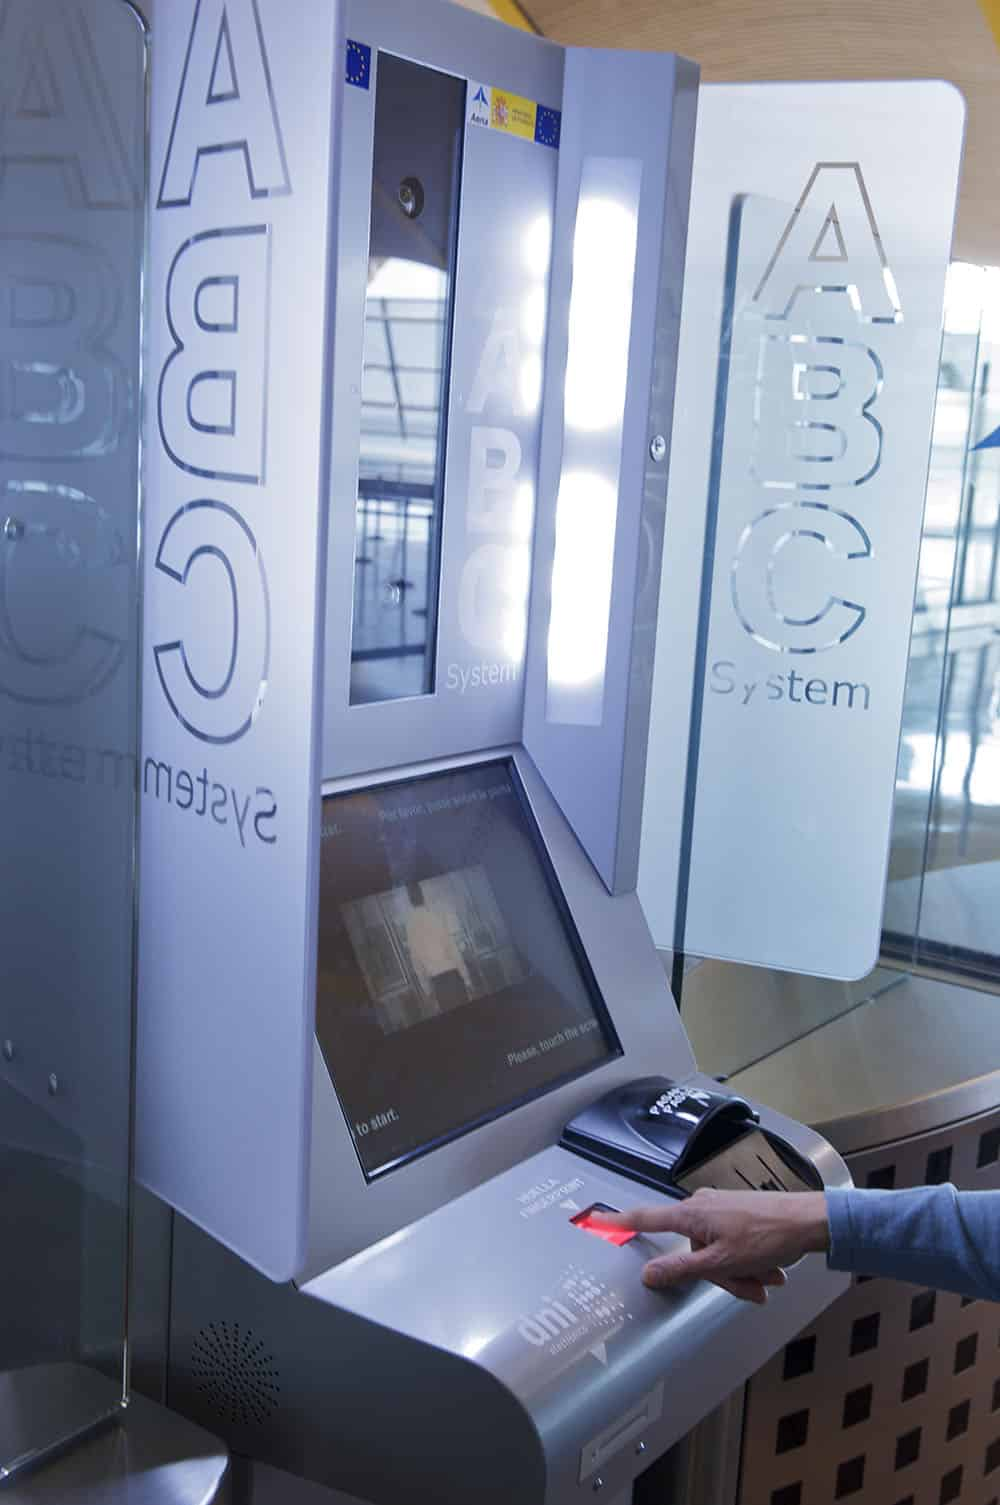
\includegraphics[width=1.0\textwidth]{informatica/ejemplo_abc_system_02}
	\end{subfigure}

	\caption{Máquinas \textit{ABC System} para realizar el control de pasaportes en aeropuertos de forma automática. Entre otras tareas, verifican que la fotografía del pasaporte se corresponda con una imagen tomada por la cámara de la máquina. Imágenes extraídas de \cite{informatica:articulo_abc_system}}
\end{figure}
\todo{Arreglar la relación de aspecto de estas imágenes}

Todo esto justifica el interés en disponer de un modelo que resuelva la tarea que hemos propuesto.

\section{Descripción de los objetivos}

Los objetivos del presente trabajo son los siguientes:

\begin{enumerate}
	\item Realizar una \textbf{revisión del estado del arte} en el ámbito del \textit{AIFR} (véase el \sectionref{ich:estado_arte}).
	\item Realizar un \textbf{estudio de los \textit{datasets}} disponibles (véase la \sectionref{isec:base_datos_usada}).
	\item \textbf{Implementar todos los módulos necesarios} para poder aplicar las técnicas a estudiar, a partir del uso de patrones de diseño para acabar con una arquitectura limpia y cómoda de trabajar (véase el \sectionref{ich:implementacion}).
	\item Llevar a cabo el proceso de \textbf{aprendizaje de un modelo profundo} que resuelva la tarea de \textit{AIFR} (véase el \sectionref{ich:Experimentación}).
	\item \textbf{Estudiar los resultados obtenidos} por dicho modelo, comparándolos con los resultados obtenidos en otros trabajos del mismo ámbito.
\end{enumerate}
\todo{Revisar esto al terminar el borrador porque he podido cambiar de sitio algunas secciones}

\section{Planificación} \label{isec:planificacion}

Tras un estudio inicial de los \textit{frameworks} de aprendizaje automático existentes, nos damos cuenta de que no hay implementaciones para las técnicas que queremos explorar. Esto supone que \textbf{deberemos dedicar un gran esfuerzo al diseño, implementación, optimización y validación de módulos de código}. Por tanto, decidimos realizar un \textbf{desarrollo en varias etapas}, iterando sobre distintas bases de datos. Empezamos trabajando con conjuntos de datos de menor interés y complejidad (estructura de los datos, facilidad de trabajo con ellos y tamaño), llegando al final a trabajar con los conjuntos de datos más complejos y relevantes para nuestro estudio. Como veremos en la \sectionref{isec:optimizacion_codigo}, esto permite desarrollar rápidamente una amplia base de código sin preocuparnos de realizar optimizaciones prematuras y poco relevantes. Solo se realiza un proceso de optimización cuando encontramos problemas reales de eficiencia. Una vez analizados y resuelto los puntos débiles en temas de rendimiento sobre conjuntos de datos sencillos, pasamos a tratar con los conjuntos que realmente nos interesan, centrándonos únicamente en la experimentación. Las bases de datos sobre las que iteramos se describen en detalle en la \sectionref{isec:base_datos_usada}.

Además, como veremos en el \sectionref{ich:estado_arte}, \textbf{no existen trabajos previos que hayan aplicado nuestro enfoque para resolver el problema de \textit{AIFR}}. Por tanto, esperamos encontrarnos con dificultades desconocidas, tanto en la implementación como en la experimentación, que deberemos resolver sin tener literatura específica sobre la que apoyarnos. Todo esto justifica que no escojamos un modelo de desarrollo en cascada clásico: no sabemos cuándo nos vamos a enfrentar con problemas de rendimiento y, por la falta de literatura, desconocemos los posibles problemas que pueden ir apareciendo. Por lo tanto, \textbf{decidimos usar un modelo de desarrollo iterativo} \cite{informatica:libro_metodologias_desarrollo}. En este modelo de desarrollo, realizamos varias iteraciones, en cada una de las cuales aplicamos el modelo en cascada. Este procedimiento encaja perfectamente con nuestro enfoque basado en iterar varios conjuntos de datos. El funcionamiento de este modelo se explica mejor en la siguiente imagen:

\begin{figure}[H]
	\centering
	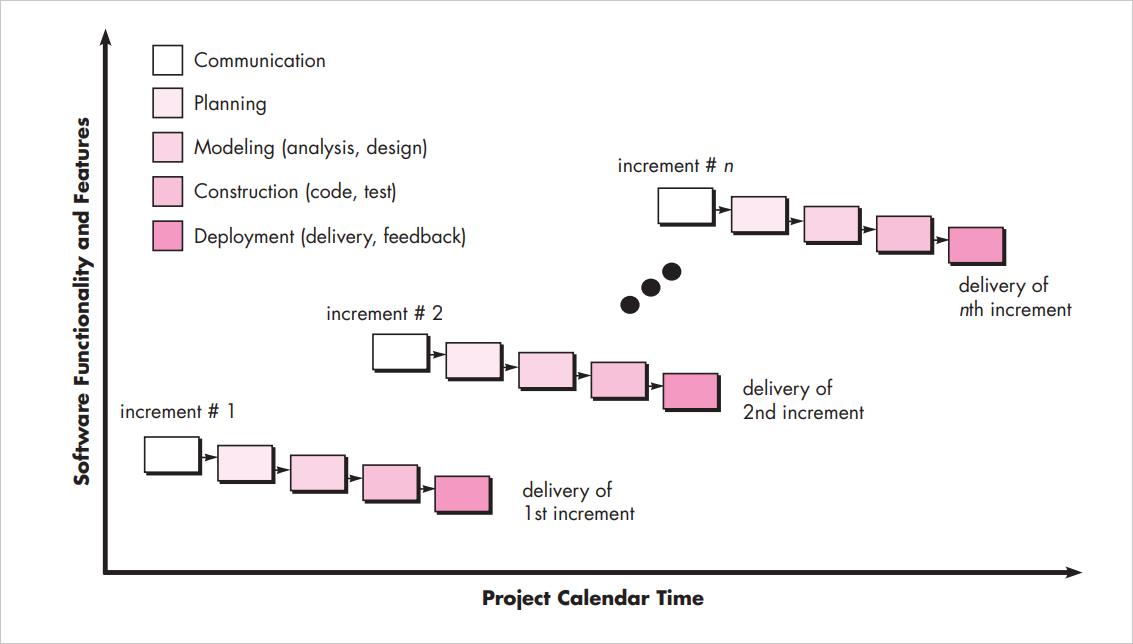
\includegraphics[width=0.8\textwidth]{informatica/ejemplo_modelo_incremental}
	\caption{Ejemplo del modelo de desarrollo incremental. Podemos ver que en cada iteración aplicamos un modelo de desarrollo en cascada. En nuestro caso, cada iteración corresponderá con cada una de las bases de datos sobre las que trabajamos. Imagen extraída de \cite{informatica:libro_metodologias_desarrollo}.}
\end{figure}

Para cada base de datos sobre la que trabajamos, consideramos las siguientes fases del modelo en cascada:

\begin{itemize}
	\item \textbf{Análisis}: realizamos un análisis exploratorio de la base de datos con la que trabajamos en esta iteración (véase la \sectionref{isec:base_datos_usada}). Estudiamos las técnicas que queremos aplicar y nos marcamos una serie de objetivos para esta iteración.
	\item \textbf{Diseño}: en base al estudio realizado y las técnicas que queremos aplicar, definimos qué módulos de código debemos de introducir, qué interfaces se deben cumplir para interactuar con otros módulos, las propiedades que queremos verificar en los \textit{tests} y distintos \textit{pipelines} que seguir en la experimentación.
	\item \textbf{Implementación}: desarrollamos el código necesario para cumplir con el diseño realizado previamente. En esta fase también incluimos el desarrollo de \textit{tests} para realizar las validaciones.
	\item \textbf{Optimización}: en esta fase realizamos \textit{profiles} para detectar partes críticas del código, introducimos \textit{benchmarks} para estudiar el impacto de los cambios realizados y llevamos a cabo dichos cambios. Esto se explica en detalle en la \sectionref{isec:optimizacion_codigo}. Esta fase es opcional, no se realiza salvo que en la iteración se detecten problemas de rendimiento relevantes.
	\item \textbf{Experimentación}: lanzamos los \textit{pipelines} desarrollados en la fase anterior (véase la \sectionref{isec:pipeline}), analizamos los resultados obtenidos y buscamos anomalías en el proceso o en los resultados. Esta fase es fundamental a la hora de marcar los objetivos y problemas a resolver en la siguiente iteración sobre una nueva base de datos.
\end{itemize}

Para organizar todas las tareas de cada iteración usamos la \textbf{metodología \textit{Kanban}} \cite{informatica:kanban_paper}. En dicha metodología se usa un tablero, en el que tarjetas que representan tareas a realizar se colocan sobre columnas que representan distintos estados. Usamos cuatro estados:

\begin{enumerate}
	\item \textit{Backlog} o tareas que no sabemos si vamos a llevar a cabo.
	\item \textit{To-do} o tareas que debemos llevar a cabo.
	\item \textit{In-progress} o tareas en las que actualmente estamos trabajando.
	\item \textit{Done} o tareas que ya se han completado.
\end{enumerate}

Esto permite tener una visualización rápida del estado de la iteración. Como comentaremos detalladamente en la \sectionref{isec:github_buenas_practicas}, usaremos la utilidad de proyectos que ofrece \textit{Github} para tener acceso a un tablero \textit{kanban}. En la siguiente imagen se muestra un ejemplo del estado de este tablero:

\begin{figure}[H]
	\centering
	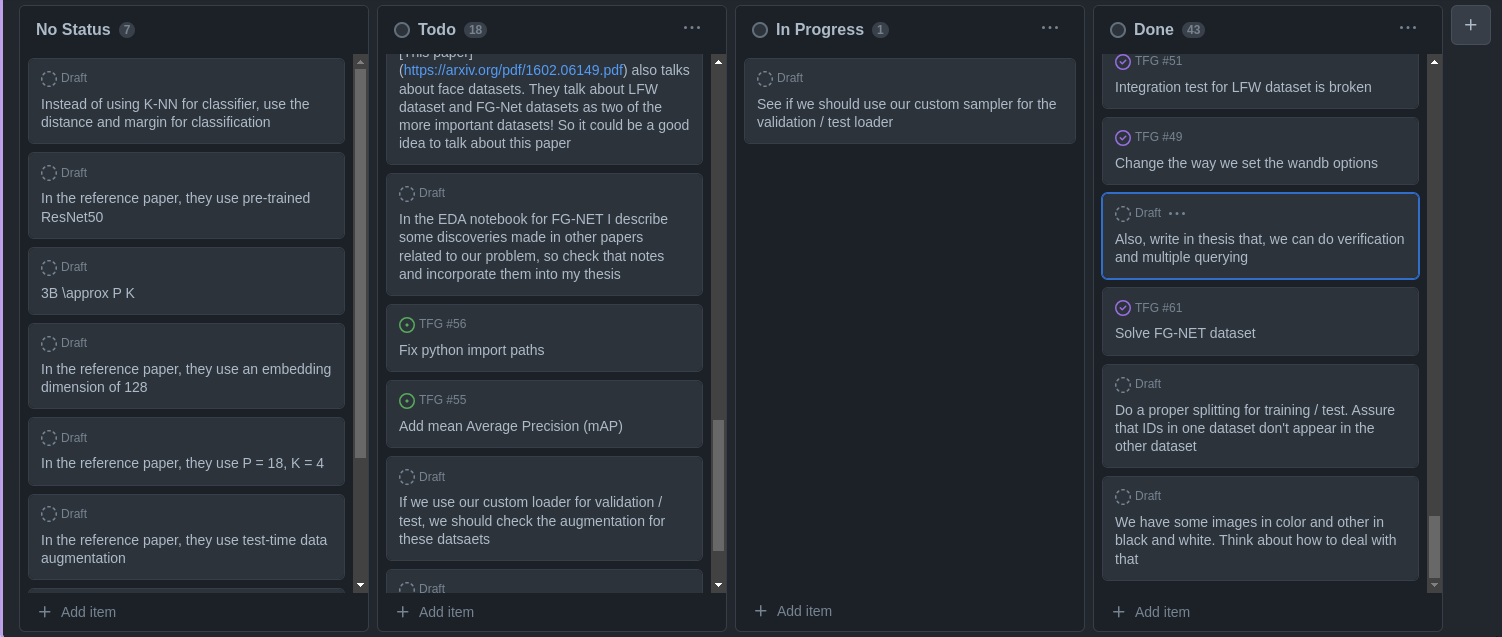
\includegraphics[width=1.05\textwidth]{informatica/kanban_board}
	\caption{Ejemplo del estado de nuestro tablero \textit{kanban} en un momento concreto durante la fase de desarrollo. Podemos ver las cuatro columnas que ya hemos descrito. \textit{Github} le da el nombre \textit{No Status} a la columna que nosotros usamos como \textit{backlog}}
\end{figure}

Comenzamos a desarrollar el proyecto en Febrero de 2022. Sabemos que, debido a los exámenes universitarios, apenas trabajaremos en los meses de Enero, Mayo y Junio. Por tanto, consideraremos que en estos meses no trabajemos ninguna hora (aunque en la práctica sí que consigamos sacar algo de tiempo). Los meses en los que más trabajaremos serán Febrero, Julio, Agosto y Septiembre. En estos meses tenemos previsto trabajar al menos 20 horas semanales. En el resto de meses consideramos que trabaremos al menos 2 horas semanales. Por tanto, en los dos años que dedicamos al proyecto de informática, dedicaremos al menos 720 horas. Teniendo todo esto en cuenta, inicialmente planificamos el proyecto tal y como describe el siguiente diagrama de Gannt:

\begin{figure}[H]
	\centering
	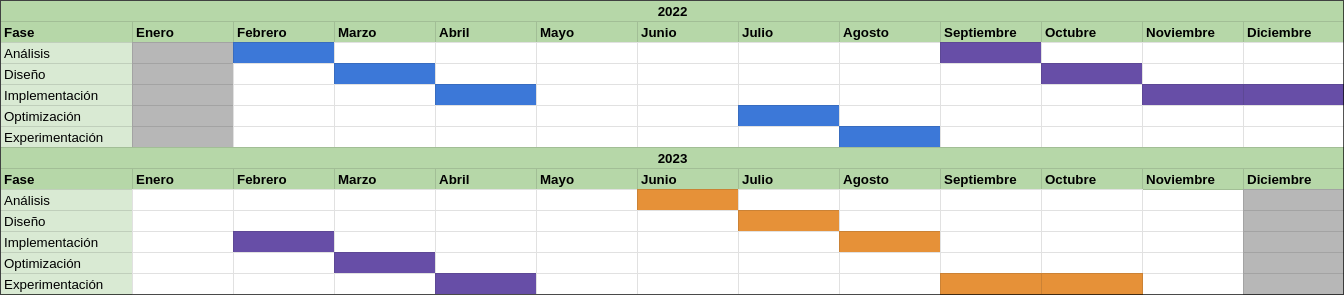
\includegraphics[width=1.0\textwidth]{informatica/diagrama_gannt_ideal}
	\caption{Diagrama de \textit{Gantt} que describe la planificación original del proyecto. El color azul corresponde al conjunto de datos \textit{MNIST}. El color morado corresponde al conjunto de datos \textit{LFW}. El color naranja corresponde a los conjuntos de datos \textit{FG-Net} y \textit{CACD}. Estas bases de datos se describen en detalle en la \sectionref{isec:base_datos_usada}.}
\end{figure}

Sin embargo, por los problemas enfrentados durante el desarrollo, y por inexactitudes en la planificación, acabamos distribuyendo el tiempo dedicado al trabajo tal y como se muestra en el siguiente diagrama de Gannt:

\begin{figure}[H]
	\centering
	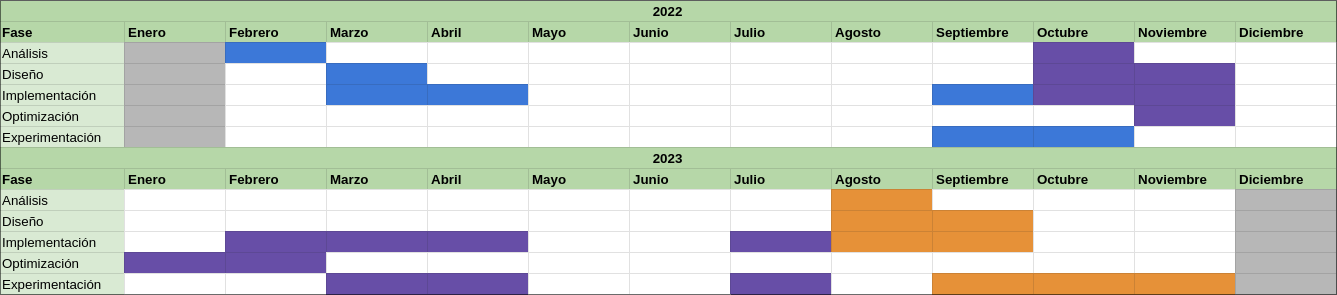
\includegraphics[width=1.0\textwidth]{informatica/diagrama_gannt_real}
	\caption{Diagrama de \textit{Gantt} que describe la distribución real del tiempo dedicado al proyecto. Seguimos el mismo código de colores que en el diagrama anterior.}
	\label{img:gannt_real}
\end{figure}

En el repositorio abierto de \textit{Github} \cite{informatica:repogithub} donde hemos desarrollado el proyecto, podemos verificar los tiempos que aparecen en \imgref{img:gannt_real} \footnote{Recordamos que explicamos en detalle el uso de \textit{Git} en la \sectionref{isec:github_buenas_practicas}.}. En cuanto a la planificación económica, tenemos en cuenta los siguientes aspectos:

\begin{itemize}
	\item El salario aproximado de un investigador en Ciencia de Datos y Aprendizaje Automático es de 35 €/h. Teniendo en cuenta que hemos dedicado al menos 720 horas de trabajo, esto supone un coste de 25.200€.
	\item El valor del ordenador que hemos usado para trabajar: 600€.
	\item El valor de los servidores \textit{nGPU} donde se han lanzado los procesos (véase la \sectionref{isec:entorno_ejecucion}). Se estima un coste de unos 145€ semanales. Teniendo en cuenta que hemos tenido acceso desde Marzo de 2023, y usamos estos servidores hasta Octubre de 2023, esto supone un coste de 4.640€.
\end{itemize}

Todo esto supone un \textbf{coste total} de unos 30.440€.

% TODO -- seguir por aqui
\section{Estructura del trabajo}

Hemos estructurado la parte informática del presente trabajo en los siguientes capítulos:

\begin{itemize}
	\item \sectionref{ich:introduccion}: introducimos el problema, lo describimos y motivamos. Comentamos los objetivos de esta parte del trabajo. Mostramos la planificación realizada y esta estructuración.
	\item \sectionref{ich:fundamentos_teoricos}: desarrollamos todos los conceptos teóricos necesarios para entender cómo hemos solucionado el problema planteado. Introducimos conceptos básicos del aprendizaje automático y aprendizaje profundo y definimos algunas técnicas más avanzadas, entre las que se encuentran ciertas variantes técnicas que son objeto principal de nuestro estudio.
	\item \sectionref{ich:estado_arte}: mostramos el interés de la comunidad científica en este área de estudio y estudiamos los trabajos que mejores resultados han obtenido.
	\item \sectionref{ich:materiales_metodos}: describimos los conjuntos de datos empleados, el entorno donde ejecutamos la experimentación y qué técnicas, tanto específicas de aprendizaje automático como de otros ámbitos de las ciencias de la computación, hemos empleado para resolver nuestro problema.
	\item \sectionref{ich:implementacion}: explicamos en profundidad cómo hemos implementado la solución al problema, cómo hemos estructurado el código para obtener una arquitectura limpia y cómoda de trabajar y cómo hemos llevado a cabo el proceso de optimización de ciertas partes del código.
	\item \sectionref{ich:Experimentación}: explicamos los protocolos de experimentación seguidos, los resultados obtenidos y qué conclusiones obtenemos a partir de estos resultado.
	\item \sectionref{ich:conclusiones}: comentamos las conclusiones obtenidas a partir de todo el trabajo realizado.

\end{itemize}

\todo{Revisar esto antes de enviar el borrador porque seguramente haya cambiado bastante la estructura del trabajo}
